\documentclass[letterpaper,12pt]{book}
\usepackage[utf8]{inputenc}
\usepackage[spanish]{babel}
\usepackage{amsmath}
\usepackage{amssymb}
\usepackage{hyperref}
\usepackage{graphicx}
\title{Clasificación de Series de Tiempo Astronómicas}
\author{Muriel Pérez\\ 201011755}
\begin{document}
\maketitle
\tableofcontents 
\chapter{Introducción}

Con los avances en técnicas de observación astronómica que han sucedido en los últimos años, hay grandes cantidades de datos disponibles. Por ejemplo se espera que el \textit{VISTA Variables in the Via Lactea} (VVV) del \textit{European Southern Observatory} (ESO) produzca del orden de $10^{9}$ curvas de luz\footnote{\label{nota:curvasDeLuz} La curva de luz de una estrella es el resultado de medir su magnitud como función del tiempo. La magnitud de una estrella es el flujo de energía observado en una parte del espectro electromagnético (una banda), delimitada por un filtro, en escala logarítmica (ver el capítulo 4 de \cite{karttunen_fundamental_2007}).} de fuentes puntuales en el infrarojo cercano con hasta 100 observaciones en diferentes épocas de alta calidad. De la misma forma estudios como la misión Kepler de la \textit{National Aeronautics and Space Administration} (NASA), cuyo objetivo principal es la detección de exoplanetas,  tienen como subproductos gran cantidad de curvas  de luz. 

Para que estos datos sean útiles para la comunidad científica es necesario clasificarlos y extraer sus características. Aunque los métodos automáticos muchas veces no pueden igualar la inspección manual por parte de un experto, la cantidad de datos disponible hace que esta tarea no sea posible en corto tiempo y hace necesario utilizar técnicas de minería de datos. Este interés se manifiesta en proyectos como el \textit{VVV Templates Project} que tiene como objetivo consolidar una base bien definida de curvas de luz de estrellas variables en el infrarojo cercano para ser utilzadas como referencia para la clasificación automática de curvas de luz.

Debido a limitaciones en el tiempo de observación, fallas técnicas, periodos de matenimiento de los instrumentos utilizados y la imposibilidad de abservar todas las regiones del cielo durante todo el año, las curvas de luz no constan del mismo número de observaciones y éstas no son hechas en intervalos regulares. Como el tiempo durante el cual cada estrella no es observada no es predecible y en ellos no se observan características importantes de las curvas de luz,  estas no pueden ser analizadas con técnicas clásicas de análisis de series de tiempo.

En estudios previos \cite{debosscher_automated_2007, sarro_automated_2009, richards_machine-learned_2011} se le ha asignado a cada curva de luz un vector, llamado vector de características, y, basado en este vector, se ha hecho la clasificación automática. La escogencia de el vector de características es crucial para el proceso de clasificación porque con él se debe poder clasificar cada curva de luz, es decir, debe logar que, en el espacio de características las clases se superpongan lo menos posible. Para la conformación de este vector se han elegido coeficientes de Fourier de la curva de luz\cite{debosscher_automated_2007, sarro_automated_2009, richards_machine-learned_2011}, que son calculados mediante métodos como el periodograma de  Lomb-Scargle \cite{scargle_studies_1982} o la minimización de la entropía de Shannon de la gráfica de la curva \cite{cincotta_astronomical_1995}. 

Esta elección de caracterísicas no es del todo conveniente porque requiere de gran poder computacional y limita el tipo de objetos que pueden ser clasificados. El cálculo del periodogramas como el de Lomb-Scargle para curvas de luz, y en general el de los métodos utilizados en la literatura, requiere de intentar una gran cantidad de periodos candidatos a ser el periodo de la curva de luz para luego elegir el mejor. Los periodos de los objetos observados varía entre desde unos pocos minutos y varios años por lo cual se requiere probar una gran cantidad de periodos. Por un lado este es un proceso es computacionalmente intensivo, lo que limita su uso en conjuntos grandes de curvas de luz; y por otro lado no es seguro que dé como resultado el periodo real de una curva de luz, por lo que a menudo éste debe ser revisado manualmente. Además el resultado de la clasificación puede ser sensible a la calidad de las curvas de luz que sean elegidas como muestra de entrenamiento \cite{debosscher_automated_2007} y limita el estudio a fuentes periódicas.  

En \cite{rodriguez_feliciano_alisis_2012, sabogal_search_2014}, los autores notaron que algunas variables descriptivas de la serie de magnitudes de una curva de luz (como su sesgo o su curtosis) sirven para clasificar ciertos tipos de estrellas con clasificadores lineales. En este trabajo retomamos esa idea y construimos un vector de características basadas en variables tomadas de estadística descriptiva. El uso de este tipo de variables tiene las ventajas de que puede ser calculadas de manera rápida y dan como resultado un vector de caracterísicas que sive para realizar clasificación con una taza de éxito alta. Para evaluar esta aproximación al problema utilizamos una parte del Catálogo de Estrellas Variables de la tercera fase del \textit{Optical Gravitational Lensing Experiment} (OGLE III)\cite{soszynski_optical_2011-2,soszynski_optical_2010,soszynski_optical_2009-1,soszynski_optical_2011,soszynski_optical_2010-2,soszynski_optical_2008-1,soszynski_optical_2013-1,soszynski_optical_2011-1,soszynski_optical_2009,pawlak_eclipsing_2013,graczyk_optical_2011,poleski_optical_2010,soszynski_optical_2013,soszynski_optical_2010-1,soszynski_optical_2008} que contiene curvas de luz  de estrellas previamente clasificadas en seis tipos de variabilidad estelar y curvas de luz de estrellas candidatas a ser clasificadas como Be (ver cuadro \ref{cuadro:datosUsados}).

En este trabajo utilizamos k-vecinos más cercanos, árboles de clasificación, máquinas de soporte vectorial y bosques aleatorios para realizar la clasificación automática de las curvas de luz basada en nuestra elección de características. Estos clasificadores fueron elegidos porque son aproximaciones muy distintas al problema de clasificación, por su naturaleza no lineal y no paramétrica; y por el hecho de que han mostrado ser efectivos en gran cantidad de aplicaciones prácticas. 

Este documento está organizado de la siguiente forma. En el capítulo \ref{cap:losDatos} damos una descripción del conjunto de datos utilizado en este trabajo. En el capítulo \ref{cap:clasificacion} presentamos y discutimos la elección de atributos y evaluamos el desempeño de los clasificadores mediante validación cruzada. En los apéndices damos una introducción matemática del problema de aprendizaje en general y una descripción de cada uno de los algorítmos utilizados en el trabajo.




\chapter{El conjunto de Datos\label{cap:losDatos}}

Los datos utilizados en este trabajo provienen de la tercera fase del \textit{Optical Gravitational Lensing Experiment} (OGLE-III). OGLE es un proyecto de larga duración cuyo objetivo principal es la búsqueda de materia oscura mediante el aprovechamiento de lentes gravitacionales. La tercera fase del protecto comenzó en 2001 y hace uso de un telescopio de $1.3$m de diámetro localizado en el observatorio de Las Campanas, Chile\cite{udalski_optical_2004}. Uno de los principales resultados de OGLE-III es la reducción y publicación \cite{udalski_optical_2008} de las curvas de luz de objetos en el bulbo de la Galaxia, la Gran Nube de Magallanes y la Pequeña Nube de Magallanes. En este trabajo utilizamos las curvas de luz de $431 653$ objetos del catálogo de estrellas variables de OGLE-III de seis tipos de variabilidad (ver tabla \ref{cuadro:datosUsados}) al cual se puede acceder en la página del proyecto \footnote{\url{http://ogle.astrouw.edu.pl/}} y $475$ curvas de luz de estrellas candidatas a ser clasificadas como Be (ESCRIBIR DE DÓNDE FUERON TOMADAS ESTAS).

Las curvas de luz tomadas del catálogo de estrellas variables de OGLE-III se encuentran clasificadas por tipo de variabilidad estelar en un proceso que que involucró, en una etapa, la inspección manual de las curvas de luz (ver referencias en la tabla \ref{cuadro:datosUsados}) por lo cual tomaremos esta clasificación como verdadera. En este trabajo utilizamos únicamente las curvas de luz registradas en la banda I \footnote{Los objetos observados emiten radiación en una parte amplia del espectro electromagnético. Los telescopios utilizan filtros para recoger solo la radiación emitida por estos objetos en ciertas partes del espectro electromagnético. El filtro I (infrarojo) tiene un ancho de banda de 149nm y una longitud de onda efectiva de 797nm (ver \cite{karttunen_fundamental_2007})} a pesar de que también se encuentra disponible información adicional sobre las curvas de luz como sus periodos y algunos coeficientes de Fourier (ver referencias en la tabla \ref{cuadro:datosUsados}). Esta elección se debe a que el cálculo de estas cantidades es computacionalmente intensivo, no siempre se encuentran disponible y proponemos hacer la clasificación utilizando variables tomadas de estadística descriptiva.

\begin{table}
  \centering
  \caption{Conjunto de datos utilizados. BG hace referencia al Bulbo Galáctico; PNM, a la Pequeña Nube de Magallanes y GNM, a la Gran Nube de Magallanes. }
  \label{cuadro:datosUsados}  
  \begin{tabular}{rr}
    \hline
    \hline
    Tipo de variabilidad y origen & \shortstack{Número \\de Objetos}\\
    \hline
    \hline 
    RR Lyrae - BG\cite{soszynski_optical_2011-2} & 16836\\
    RR Lyrae - PNM \cite{soszynski_optical_2010}& 2475\\
    RR Lyrae - GNM \cite{soszynski_optical_2009-1}& 24906\\
    \hline
    Cefeidas - BG \cite{soszynski_optical_2011}& 32\\%El título del paper es classical and type2 cepheids
    Cefeidas - PNM \cite{soszynski_optical_2010-2}& 4630\\
    Cefeidas - GNM \cite{soszynski_optical_2008-1}& 3361\\
    \hline
    Variables de Largo Periodo - BG \cite{soszynski_optical_2013-1}& 232406\\
    Variables de Largo Periodo - PNM \cite{soszynski_optical_2011-1}& 19384\\
    Variables de Largo Periodo - GNM \cite{soszynski_optical_2009}& 91995\\
    \hline
    Sistema Binario Eclipsante - PNM \cite{pawlak_eclipsing_2013}& 6138\\
    Sistema Binario Eclipsante - GNM \cite{graczyk_optical_2011}& 26121\\
    \hline
    $\delta$-Scuti - Nube Mayor de Magallanes\cite{poleski_optical_2010} & 2786\\
    \hline
    Cefeidas Tipo II - BG \cite{soszynski_optical_2013}& 335\\
    Cefeidas Tipo II - PNM \cite{soszynski_optical_2010-1}& 43\\
    Cefeidas Tiplo II - GNM \cite{soszynski_optical_2008}& 197\\
    \hline
    Cadidata a Be -  Vía Láctea (cita!) & 475\\
    \hline
    \hline 
  \end{tabular} 
\end{table}


Agrupamos los $432128$ objetos disponibles en siete clases de variabilidad estelar (ver tabla\ref{cuadro:cantidadDatos}). Esta elección de clases puede ser refinada puesto que en cada una de estas clases existen subclases. Por ejemplo entre las Cefeidas se puede distinguir entre aquellas que pulsan en su modo fundamental, en su primer sobretono (segundo armónico) o en su segundo sobretono (tercer armónico)  (ver figura \ref{fig:tiposCefeidas}). Sin embargo conocer a qué clase de variabilidad estelar pertence un objeto facilita considerablemente su clasificación en subclases y análisis subsecuentes. 

\begin{table}[ht]
  \centering
  \caption{Cantidad de datos por tipo de variabilidad}
  \label{cuadro:cantidadDatos}
  \begin{tabular}{rrr}
    \hline
    Tipo de Variabilidad & Cantidad \\
    \hline
    Variables de Largo Periodo (VLP) & 343782 \\
    RR Lyrae (RRLyr) & 44217\\
    Cefeida (Cef)& 8004\\
    Sistema Binario Eclipsante (SBE)&32259 \\
    $\delta$-Scuti ($\delta$Sct)& 2788\\
    Cefeida Tipo II (CefT2)& 603\\
    Candidata a Be (BeEC)& 475\\
    \hline
    Total & 432128\\
    \hline
  \end{tabular}
\end{table}




\begin{figure}
  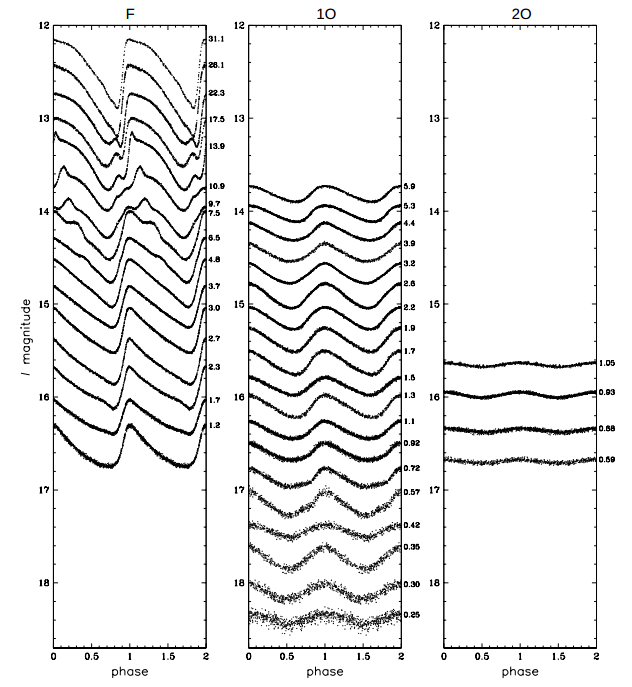
\includegraphics[width = \textwidth]{./img/C2Datos/tiposCefeidas.png}
  \label{fig:tiposCefeidas}
  \caption{Curvas de luz ilustrativas de Cefeidas en modo fundamental (izquierda), primer sobretono (mitad), segundo sobretono (derecha). Los números pequeños a la derecha de cada recuadro muestran los periodos redondeados de las curvas de luz presentadas en los recuadros. Tomado de \cite{soszynski_optical_2011}}
\end{figure}

En el Catálogo de Estrellas Variables de OGLE-III, cada curva de luz está disponible en un archivo que contiene tres columnas con los valores de magnitud, fecha juliana \footnote{La fecha Juliana es el tiempo medido en días desde el 1 de enero de 4713 a. C.} en la que fue tomada cada medida y error en la medida de la magnitud. El número de medidas para cada objeto y la separación temporal varía ampliamente. La separación mínima dos mediciones en toda la muestra es de 0.00147d, la máxima es 2156.9d y en promedio están separadas por 5.1d; por su parte el número promedio de observaciones por objeto es 759; el máximo, 5173; y el mínimo,  11. El 75\% de los objetos cuenta con más de 386 observaciones. Para todos los objetos estas observaciones están repartidas en los (número de años) años en que estuvo activo OGLE-III. En la figura \ref{fig:curvaDeLuz} se puede observar una curva de luz del catálogo de estrellas variables de OGLE-III.    

\begin{figure}
  %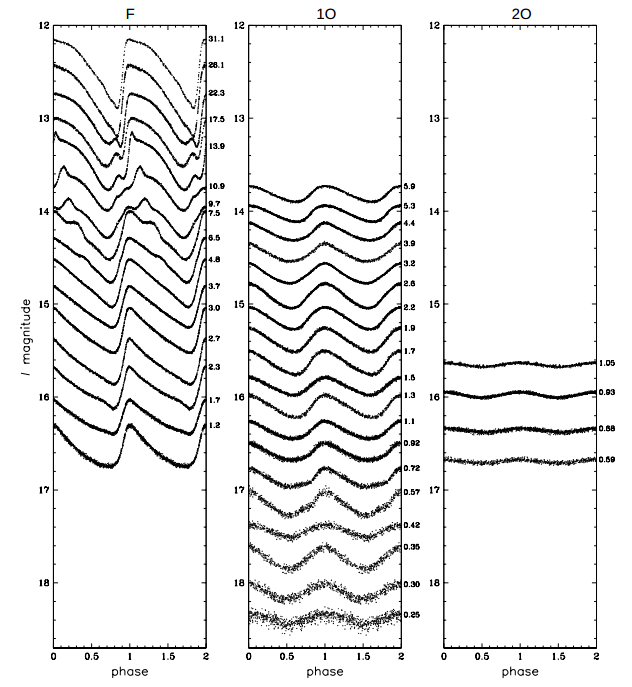
\includegraphics[width = \textwidth]{./img/C2Datos/tiposCefeidas.png}
  \label{fig:curvaDeLuz}
  \caption{(figura pendiente de imagen) Curva de luz (nombre del archivo) del catálogo OGLE-III. Los periodos en los que no hay mediciones corresponden a los momentos del año en los que la zona en la que se encuentra el objeto no puede ser observada debido a la posición relativa entre el Sol y la Tierra.}
\end{figure}

\chapter{Clasificación}\label{cap:clasificacion}



\section{Atributos Seleccionados \label{sec:atributos}}

\section{K Vecinos Más Cercanos}
\begin{table}[ht]
\centering
\caption{k = 1} 
\label{table:cmknn}
\begin{tabular}{rrrrrrrr}
  \hline
 & becand & cep & dcst & ebs & lpv & rrlyr & t2cep \\ 
  \hline
becand & 381 &   1 &   0 &  50 &  41 &   0 &   0 \\ 
  cep &   1 & 6595 &   4 & 172 &  54 & 986 &  87 \\ 
  dcst &   0 &   7 & 2064 & 340 &  13 & 151 &   0 \\ 
  ebs &  51 & 184 & 536 & 30129 & 573 & 668 &  29 \\ 
  lpv &  42 & 187 &  19 & 944 & 342740 & 371 & 158 \\ 
  rrlyr &   0 & 971 & 165 & 595 & 308 & 41911 & 217 \\ 
  t2cep &   0 &  59 &   0 &  29 &  53 & 130 & 112 \\ 
   \hline
\end{tabular}
\end{table}

\begin{table}[ht]
\centering
\caption{k=1, validación cruzada de 10 iteraciones} 
\label{table:cmCvKnn}
\begin{tabular}{rrrrrrrr}
  \hline
 & becand & cep & dcst & ebs & lpv & rrlyr & t2cep \\ 
  \hline
becand & 0.80 & 0.00 & 0.00 & 0.00 & 0.00 & 0.00 & 0.00 \\ 
  cep & 0.00 & 0.82 & 0.00 & 0.01 & 0.00 & 0.02 & 0.14 \\ 
  dcst & 0.00 & 0.00 & 0.74 & 0.01 & 0.00 & 0.00 & 0.00 \\ 
  ebs & 0.11 & 0.02 & 0.19 & 0.93 & 0.00 & 0.02 & 0.05 \\ 
  lpv & 0.09 & 0.02 & 0.01 & 0.03 & 1.00 & 0.01 & 0.26 \\ 
  rrlyr & 0.00 & 0.12 & 0.06 & 0.02 & 0.00 & 0.95 & 0.36 \\ 
  t2cep & 0.00 & 0.01 & 0.00 & 0.00 & 0.00 & 0.00 & 0.19 \\ 
   \hline
\end{tabular}
\end{table}

\section{Árboles de clasificación y regresión}
%Matriz de confusión para Cart
\begin{table}[ht]
\centering
\caption{Matriz de confusión para CART} 
\label{cuadro:cmCart}
\begin{tabular}{rrrrrrrr}
  \hline
 & becand & cep & dcst & ebs & lpv & rrlyr & t2cep \\ 
  \hline
becand & 470 &  12 &   6 & 1039 & 8906 &  47 &  18 \\ 
  cep &   0 & 6210 &  12 &  18 & 320 & 3098 &  92 \\ 
  dcst &   0 &  35 & 2511 & 5538 &  91 & 1615 &   1 \\ 
  ebs &   0 &   1 & 148 & 21346 & 346 &  64 &   1 \\ 
  lpv &   5 & 107 &  24 & 1762 & 304810 & 100 &   3 \\ 
  rrlyr &   0 & 648 &  82 & 552 & 13880 & 34313 &  92 \\ 
  t2cep &   0 & 991 &   5 & 2004 & 15429 & 4980 & 396 \\ 
   \hline
\end{tabular}
\end{table}

%Errores de validación cruzada para cart
\begin{table}[ht]
\centering
\caption{Tasas de clasificación estimadas por validación cruzada de 10 iteraciones} 
\label{table:cmCvart}
\begin{tabular}{rrrrrrrr}
  \hline
 & becand & cep & dcst & ebs & lpv & rrlyr & t2cep \\ 
  \hline
becand & 0.99 & 0.00 & 0.00 & 0.03 & 0.03 & 0.00 & 0.03 \\ 
  cep & 0.00 & 0.78 & 0.00 & 0.00 & 0.00 & 0.07 & 0.15 \\ 
  dcst & 0.00 & 0.00 & 0.90 & 0.17 & 0.00 & 0.04 & 0.00 \\ 
  ebs & 0.00 & 0.00 & 0.05 & 0.66 & 0.00 & 0.00 & 0.00 \\ 
  lpv & 0.01 & 0.01 & 0.01 & 0.05 & 0.89 & 0.00 & 0.00 \\ 
  rrlyr & 0.00 & 0.08 & 0.03 & 0.02 & 0.04 & 0.78 & 0.15 \\ 
  t2cep & 0.00 & 0.12 & 0.00 & 0.06 & 0.04 & 0.11 & 0.66 \\ 
   \hline
\end{tabular}
\end{table}

\section{Máquinas de Soporte Vectorial}

\begin{table}[ht]
\centering
\caption{$\gamma = 0.1$, costo = $16$} 
\label{table:cmSvm}
\begin{tabular}{rrrrrrrr}
  \hline
 & becand & cep & dcst & ebs & lpv & rrlyr & t2cep \\ 
  \hline
becand & 297 &   0 &   2 &  26 &  16 &   0 &   0 \\ 
  cep &   0 & 4622 &   0 &  55 &  85 & 788 &  69 \\ 
  dcst &   0 &   0 & 1683 & 163 &   4 &  47 &   0 \\ 
  ebs &  89 &  48 & 865 & 29439 & 198 & 563 &   5 \\ 
  lpv &  89 & 490 &  22 & 1380 & 342823 & 1113 & 255 \\ 
  rrlyr &   0 & 2844 & 216 & 1196 & 656 & 41706 & 274 \\ 
  t2cep &   0 &   0 &   0 &   0 &   0 &   0 &   0 \\ 
   \hline
\end{tabular}
\end{table}

\begin{table}[ht]
\centering
\caption{$\gamma = 0.1$, costo = $16$, validación cruzada de 10 iteraciones} 
\label{table:cmCvSvm}
\begin{tabular}{rrrrrrrr}
  \hline
 & becand & cep & dcst & ebs & lpv & rrlyr & t2cep \\ 
  \hline
becand & 0.63 & 0.00 & 0.00 & 0.00 & 0.00 & 0.00 & 0.00 \\ 
  cep & 0.00 & 0.58 & 0.00 & 0.00 & 0.00 & 0.02 & 0.11 \\ 
  dcst & 0.00 & 0.00 & 0.60 & 0.01 & 0.00 & 0.00 & 0.00 \\ 
  ebs & 0.19 & 0.01 & 0.31 & 0.91 & 0.00 & 0.01 & 0.01 \\ 
  lpv & 0.19 & 0.06 & 0.01 & 0.04 & 1.00 & 0.03 & 0.42 \\ 
  rrlyr & 0.00 & 0.36 & 0.08 & 0.04 & 0.00 & 0.94 & 0.45 \\ 
  t2cep & 0.00 & 0.00 & 0.00 & 0.00 & 0.00 & 0.00 & 0.00 \\ 
   \hline
\end{tabular}
\end{table}

\section{Bosques Aleatorios}


\chapter{Apéndices}

\section{El Problema del Aprendizaje\label{cap:problemaAprendizaje}}

\section{K Vecinos Más cercanos}

\section{Árboles de Clasificación y Regresión}

\section{Máquinas de Soporte Vectorial}

\section{Bosques Aleatorios}

\section{Estimación del Error de Clasificación}\label{sec:estimacionError}


\chapter{Cosas que la evolución se llevó}

\section{vieja introducción}
% En este trabajo abordamos el problema de clasificar curvas de luz de estrellas variables por su tipo de variabilidad \footnote{Las estrellas variables son estrellas cuya magnitud cambia en el tiempo (ver nota \ref{nota:curvasDeLuz}). Pueden ser periódicas o no periódicas y se pueden clasificar como pulsantes, eruptivas o variables eclipsantes aunque existen subclases de variabilidad estelar. Una estrella puede ser clasificada en estas subclases conociendo su curva de luz (ver el capítulo 13 de \cite{karttunen_fundamental_2007}).} como un problema de aprendizaje supervisado. Para esto utilizamos una parte de los resultados de la tercera fase del \textit{Optical Gravitational Lensing Experiment} (OGLE III) que contiene curvas de luz  de estrellas previamente clasificadas en seis tipos de variabilidad estelar y curvas de luz de estrellas candidatas a ser clasificadas como Be (ver capítulo \ref{cap:losDatos}) (ver cuadro \ref{cuadro:datosUsados}). 


% Para abordar el problema de clasificación adoptamos el siguiente punto de vista. Cada curva de luz $c_i = \{(t_{n}^{i}, m_{n}^{i})\}_{n}$ es una sucesión de parejas donde la primera es el tiempo y la segunda es la magnitud medida en ese instante.  Debido a limitaciones en el tiempo de observación, fallas técnicas, periodos de matenimiento de los instrumentos utilizados y el hecho de que no todas las regiones del cielo son observables durante todo el año y solo se puede observar una región limitada en cada oportunidad, las curvas de luz no constan del mismo número de observaciones y éstas no son hechas en intervalos regulares ($t_{k} - t_{k+1}$ no es constante). Una forma de hacer frente a esto es asignarle a cada curva de luz $c_i$ un vector de atributos $\vec{x_{i}} = \vec{x_{i}}(c_i)\in\mathbb{R}^{n}$ calculados a partir de de $c_i$ (ver sección \ref{sec:atributos}) que intenten describir los tipos de variabilidad. Como los elementos de la muestra han sido clasificados previamente, le asignamos a cada curva de luz $c_i$ una etiqueta $j_i\in J=\{\text{RR Lyr}, \dots, \text{BeSC}\}$ (ver tabla \ref{cuadro:datosUsados}) que corresponde al tipo de variabilidad estelar de la estrella observada.  Dicha etiqueta, a su vez, es heredada por el vector de atributos $\vec{x}_i$.

% Si nuestra elección de atributos es acertada, podremos utilizar la representación de las curvas de luz en el espacio de atributos para realizar la clasificación, esto es, existirá una función $g:\mathbb{R}^n\rightarrow J$ que, de alcanzar la mejor tasa de clasificación correcta posible para esos atributos, le asigna a cada curva de luz el tipo de variabilidad correcto con probabilidad alta (ver capítulo \ref{cap:problemaAprendizaje}). Puede suceder que, si los atributos no caracterizan los diferentes tipos de variabilidad, incluso utilizando el mejor clasificador posible (la mejor función $g$) no sea posible alcanzar errores de clasificación bajos. De esto se sigue que la elección de atributos es crucial para lograr una buena clasificación. La elección de los atributos utilizados se discute en la sección \ref{sec:atributos}.

% El siguiente problema será el de inferir (aprender) de los datos una función $\hat{g}:\mathbb{R}^n\rightarrow J$ que se aproxime tanto como sea posible a la mejor regla posible en cuanto a que maximice la probabilidad de clasificación correcta. Para encontrar esta regla existen diferentes aproximaciones y algorítmos que permiten la división del espacio de atributos en zonas a cada una de las cuales se le asigna un tipo de variabilidad. En la práctica no se conoce la mejor regla posible porque esto requeriría el conocimiento de la distribución exacta de los atributos (ver capítulo \ref{cap:problemaAprendizaje}). Tampoco se conoce el mínimo error de clasificación posible por lo que, para la selección del mejor clasificador entre los posibles, se utilizan estimaciones del error de clasificación que utilizan la muestra disponible, en este caso validación cruzada (ver sección \ref{sec:estimacionError}).En el capítulo \ref{cap:aprendizaje} utilizamos k vecinos más cercanos, arboles de clasificación y regresión; y maquinas de soporte vectorial para inferir la función $\hat{g}$. Asímismo analizamos los estimados de la probabilidad de error al usar cada algorítmo y comentamos las ventajas comparativas de cada uno. Estos tres métodos son muy diferentes en su naturaleza, fueron elegidos porque han mostrado ser efectivos en gran variedad de aplicaciones y por su carácter no paramétrico y no lineal. 

% Así la clasificación de una curva de luz correspondiente a una estrella cuyo tipo de variabilidad es desconocido será un proceso de dos pasos. El primero será la extracción de los atributos. El segundo paso será la clasificación basada en los atributos utilizando la función $\hat{g}$ que fue encontrada con ayuda de la muestra disponible. Esta clasificación será correcta con cierta probabilidad, estimada con validación cruzada.

% Este documento está organizado de la siguiente manera. En el capítulo \ref{cap:losDatos} damos un análisis descriptivo del conjunto de datos que consideramos y discutimos la elección de los atributos para realizar la clasificación. En el capítulo \ref{cap:problemaAprendizaje} discutimos brevemente el problema de clasificación en general, describimos el mejor clasificador posible (el clasificador de Bayes), discutimos la imposibilidad de utilizarlo en la mayoría de aplicaciones complejas y describimos el método que usamos para estimar la probabilidad de error de los clasificadores. En el capítulo \ref{cap:aprendizaje} describimos los métodos de clasificación utilizados, damos los estimados del error de clasificación y comparamos los resultados con otros valores dados en la literatura.

\bibliographystyle{plain}
\bibliography{tesisMatematicas}

\end{document}